\documentclass[10pt]{exam}
\usepackage[phy]{template-for-exam}
\usepackage{graphicx}
\usepackage{caption,multicol,tikz}
\usetikzlibrary{decorations.markings}

\title{ReFRACtion Lab (MAKEUP Version if Absent)}
\author{Rohrbach}
\date{\today}

\begin{document}
\maketitle

\noindent
{\small \it This lab is based on Experiment \#4 in PASCO's Introductory Optics System Manual.}

\section*{Purpose} To observe what happens to rays of light refract at a lens

\vspace{-1em}

\section*{Procedure}
\begin{enumerate}
  \item Go to \texttt{phet.colorado.edu}.  Type in ``\emph{bending light}'' into the search bar.  Make sure that you are using the HTML5 simulation.
  \item	Click play.  Then click “More Tools”
  \item	Make sure the checkboxes in the lower left corner labeled “Normal” and “Angles” are checked.
  \item Turn on the laser and then drag it to change the angle of incidence. 
  \item Set up the simulation so that the laser is traveling from air to glass.  Measure the angles of refraction and reflection for each angle of incidence (Figure~\ref{ag}).
  \item Flip the simulation so that the laser is traveling from glass to air.  Measure the angles of refraction and reflection for each angle of incidence (Figure~\ref{ga}).
  
\end{enumerate}

\noindent
\begin{figure}[h]
  \centering
  \begin{minipage}[b]{8cm}
    \centering
    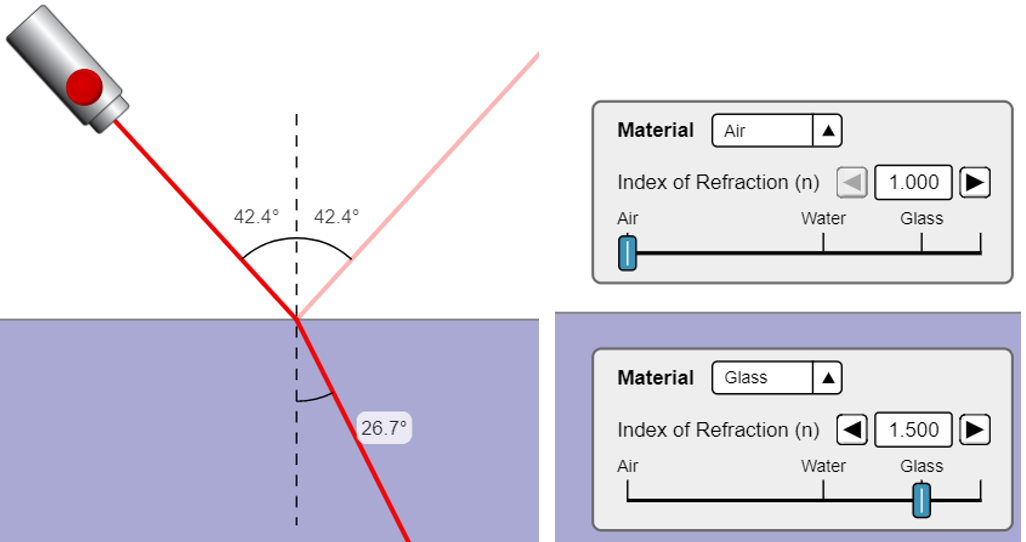
\includegraphics[width=8cm]{AG.png}
    \captionof{figure}{Air $\rightarrow$ Glass}
    \label{ag}
  \end{minipage}%
  \begin{minipage}[b]{8cm}
    \centering
    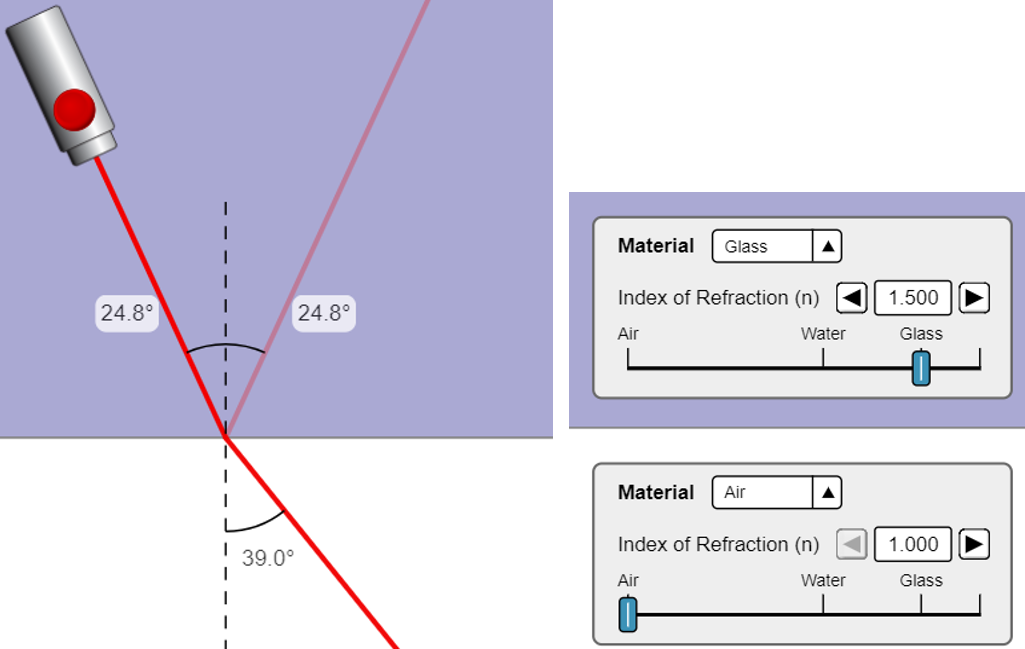
\includegraphics[width=8cm]{GA.png}
    \captionof{figure}{Glass $\rightarrow$ Air}
    \label{ga}
  \end{minipage}
\end{figure}


\pagebreak

\section*{Data}

\emph{Not all of the rays will be visible.  If a ray is not visible, write ``{\bf n.v.}'' for ``not visible.''}

\renewcommand{\arraystretch}{1.7}

\begin{multicols}{2}
  \begin{tabular}{|c|c|c|}
    \hline
    \multicolumn{3}{|c|}{Angles for {\bf Air $\rightarrow$ Glass}} 
    \\\hline
    Incidence &
    Refraction &
    Reflection \\\hline
    $10^\circ$ && \\\hline
    $20^\circ$ && \\\hline
    $30^\circ$ && \\\hline
    $40^\circ$ && \\\hline
    $50^\circ$ && \\\hline
    $60^\circ$ && \\\hline
    $70^\circ$ && \\\hline
    $80^\circ$ && \\\hline
  \end{tabular}

  \columnbreak

  \begin{tabular}{|c|c|c|}
    \hline
    \multicolumn{3}{|c|}{Angles for {\bf Glass $\rightarrow$ Air}} 
    \\\hline
    Incidence &
    Refraction &
    Reflection \\\hline
    $10^\circ$ && \\\hline
    $20^\circ$ && \\\hline
    $30^\circ$ && \\\hline
    $40^\circ$ && \\\hline
    $50^\circ$ && \\\hline
    $60^\circ$ && \\\hline
    $70^\circ$ && \\\hline
    $80^\circ$ && \\\hline
  \end{tabular}


\end{multicols}

\vspace{-1em}
\begin{questions}

\uplevel{\section*{Analysis}}

  \question
    The results of the two trials ({\bf Air $\rightarrow$ Glass} and {\bf Glass $\rightarrow$ Air}) are not the same.  What pattern do you notice with the angles of refraction? (\emph{i.e.} Are they larger or smaller than the angle of incidence?)
    \vs
  
  \question
    What difficulties did you have at large angles?  Why do you think these difficulties arose?
    \vs 
  
  \question
    What did you notice about the angle of reFLECtion?
    \vs 



\end{questions}




\end{document}